\documentclass[11pt,a4paper]{ctexart}
\usepackage[margin=2.4cm]{geometry}
\usepackage{graphicx}
\usepackage{booktabs}
\usepackage{amsmath}
\usepackage{hyperref}

\title{反光焦堆仿真的超分辨下采样策略分析}
\author{SRTP Project Notes}
\date{2026-06-21}

\begin{document}
\maketitle

\section{问题定义}

反光表面焦堆仿真存在一个容易被忽视的数值问题：若直接在相机输出分辨率上生成高度图、计算法线和镜面反射，局部斜率会受到网格分辨率强烈影响，可能产生像素级伪眩光。更合理的流程是在高分辨率微几何上计算法线、反射、离焦和曝光，再积分下采样到相机像素尺度。

\section{对比路径}

本文比较两条仿真路径：

\begin{itemize}
  \item \textbf{direct\_lowres}: 先把高度图降到相机分辨率，再计算法线、glare risk 和焦堆。
  \item \textbf{superres\_integrated}: 在 2x/4x/8x 高分辨率上计算微几何和焦堆，再 block-average 到相机分辨率。
\end{itemize}

\section{结果}

\begin{table}[htbp]
\centering
\small
\begin{tabular}{rllrrrr}
\toprule
Factor & Mode & Risk mean & High risk & Max p99 & Max sat. & Best Lap. \\
\midrule
2 & superres & 0.0035 & 0.0000 & 0.8317 & 0.0000 & 8 \\
2 & direct & 0.0063 & 0.0054 & 0.8612 & 0.0031 & 12 \\
4 & superres & 0.0020 & 0.0000 & 0.8162 & 0.0000 & 8 \\
4 & direct & 0.0072 & 0.0065 & 0.8696 & 0.0039 & 12 \\
8 & superres & 0.0011 & 0.0000 & 0.7968 & 0.0000 & 9 \\
8 & direct & 0.0113 & 0.0100 & 0.8884 & 0.0063 & 12 \\
\bottomrule
\end{tabular}
\caption{Direct low-resolution simulation versus super-resolution-integrated simulation.}
\end{table}

\begin{figure}[htbp]
\centering
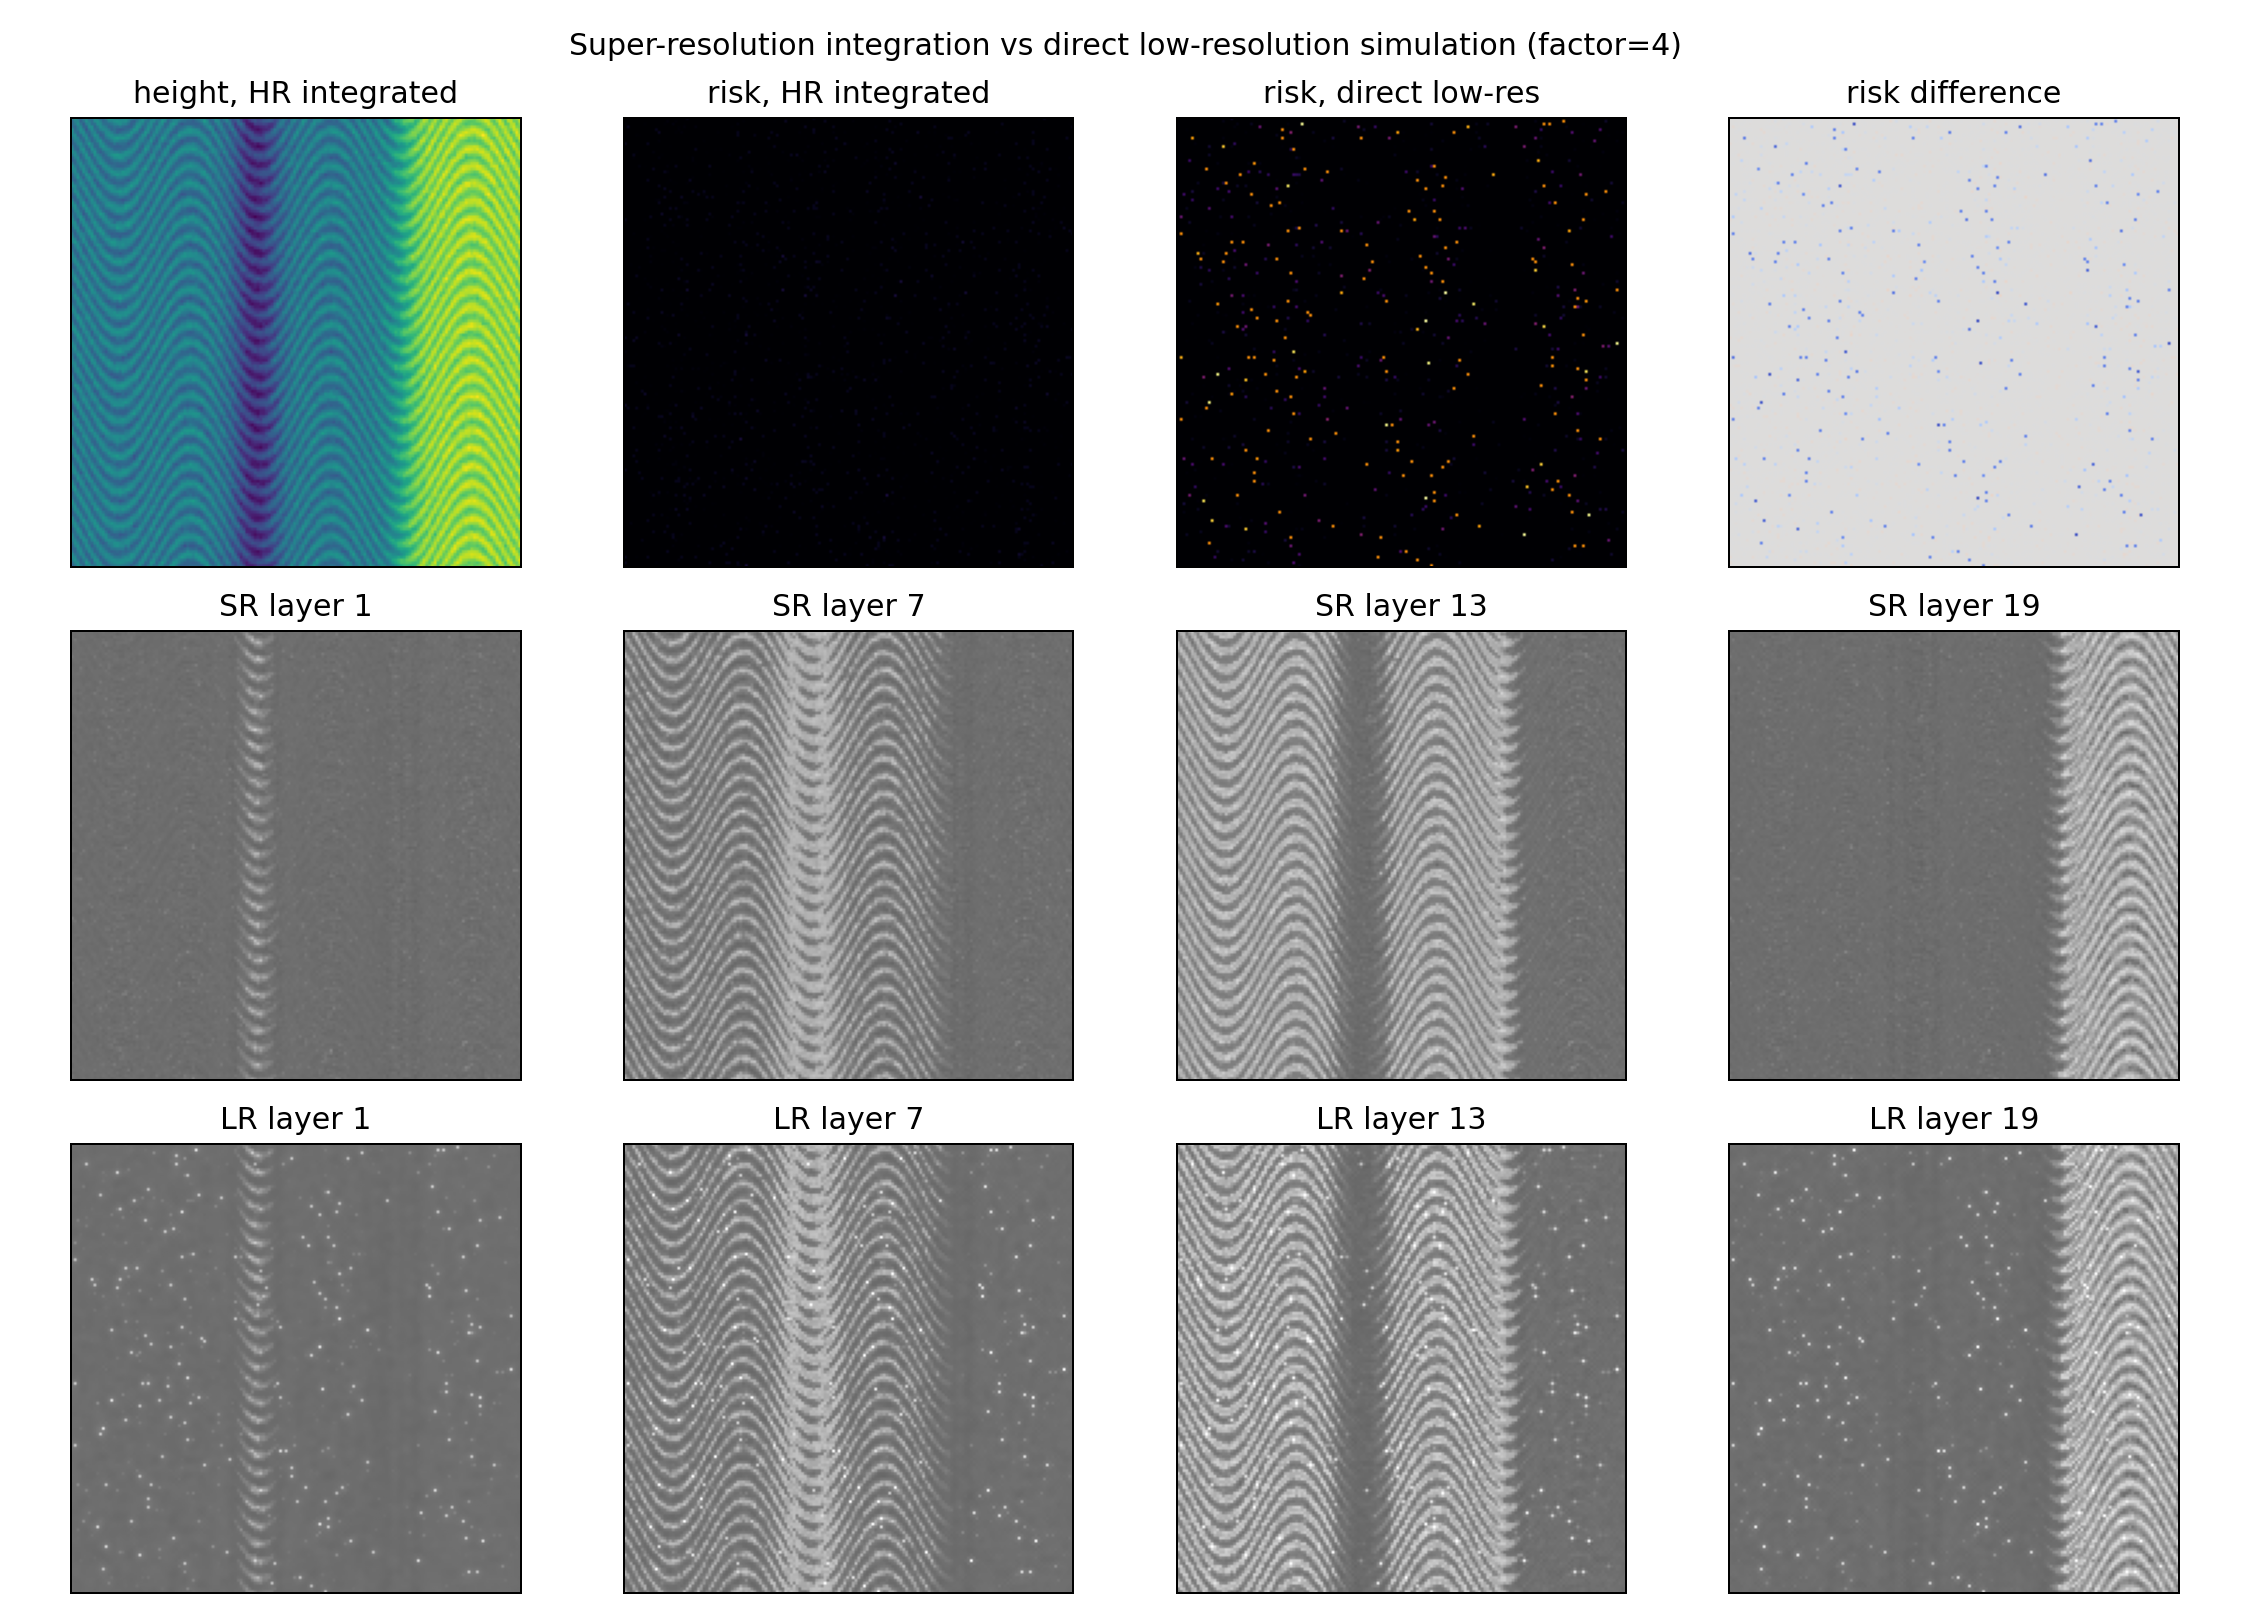
\includegraphics[width=0.95\linewidth]{superres_sampling_branch/sr_factor_4_comparison_panel.png}
\caption{4x super-resolution integration versus direct low-resolution simulation. Direct low-resolution computation introduces many pixel-level bright artifacts.}
\end{figure}

\begin{figure}[htbp]
\centering
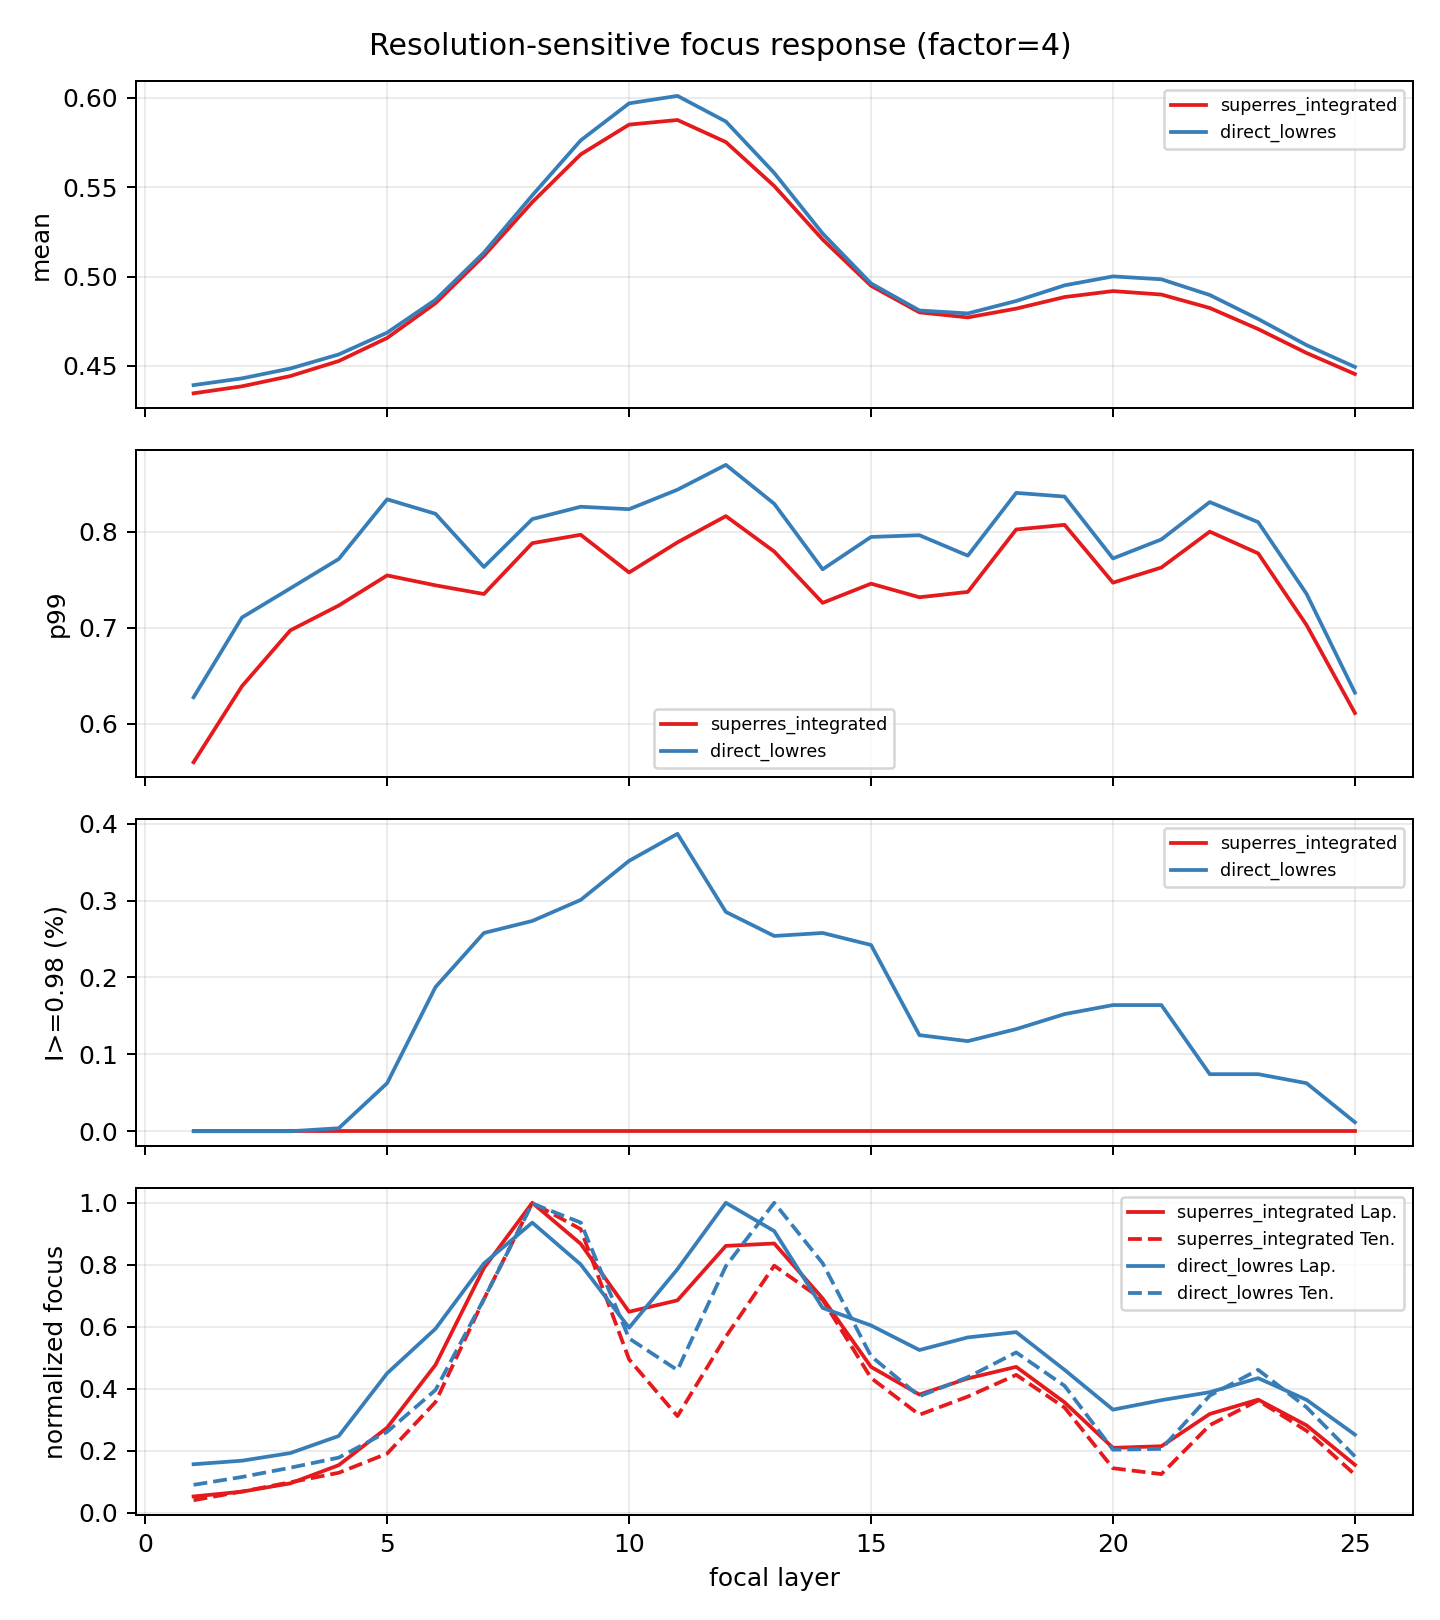
\includegraphics[width=0.95\linewidth]{superres_sampling_branch/sr_factor_4_curves.png}
\caption{Resolution-sensitive focus response. Direct low-resolution simulation raises p99 and near-saturation ratio and shifts focus-response peaks.}
\end{figure}

\section{机理解释}

高度图法线计算为
\begin{equation}
\mathbf{n}=\mathrm{normalize}[-\partial z/\partial x,\ -\partial z/\partial y,\ 1].
\end{equation}
若在低分辨率上计算 $\partial z/\partial x$ 和 $\partial z/\partial y$，微结构边缘、划痕和粗糙纹理会被少数像素代表，局部法线可能被过度倾斜或错误平滑。由于镜面反射方向高度依赖法线，低分辨率法线误差会转化为 glare-risk 误差。

真实相机像素对应有限感光面积内的光强积分。对反光微结构而言，一个像素内可能同时包含高风险和低风险微面。因此，先在高分辨率上计算反射和离焦，再进行像素积分下采样，比直接低分辨计算更接近实际成像。

\section{建议流程}

\begin{enumerate}
  \item 在目标相机分辨率的 4x 或 8x 上生成微米级高度图。
  \item 在高分辨率上计算 normal map、glare-risk map、texture、defocus PSF 和 exposure clipping。
  \item 使用 block-average 或 pixel aperture kernel 下采样到 sensor resolution。
  \item 在 sensor resolution 上运行 DFF/GADFF 和深度网络。
  \item 同时保存 downsampled mean risk 与 max risk，分别表示平均风险和子像素极端风险。
\end{enumerate}

\section{论文可用表述}

\begin{quote}
To avoid grid-dependent specular artifacts, synthetic focal stacks are generated at a super-resolved microgeometry resolution and then integrated to the sensor resolution. Surface normals, glare-risk maps, defocus blur, and exposure clipping are computed before downsampling, so that each sensor pixel approximates an area integral over subpixel microfacets.
\end{quote}

\section{结论}

仿真到真实的差距不只来自材质、光照或纹理分布，也可能来自仿真器的数值采样策略。对于反光微结构，直接低分辨仿真会放大局部法线误差并制造伪高亮；超分辨微几何计算加像素积分下采样是更稳健的默认策略。

\end{document}
